%-------------------------------------------------------------------------------
\section{Design}
%-------------------------------------------------------------------------------
\sys{} models an application's schema as a graph of data \emph{entities}. Each entity type corresponds to
an application data table, such as stories, users, or votes. 
Entities are linked in the entity graph by foreign key relationships: table columns that act as foreign keys to other tables create child-parent relationships between
entities.
\sys{} also includes abstract entities in the graph, where the keys may be non-referential
identifiers that refer to abstract, non-table entities (e.g.,\ a \texttt{thread\_id} column in the
comments table).
Edges in the graph---foreign or abstract key relationships---represent correlations between the nodes of the graph,
namely individual entities.

\subsection{Specifying Decorrelation Policies}
The developer provides a two-part specification to \sys{}: 
\begin{enumerate}
    \item Ghost entity generation policies on entity types, and
    \item Decorrelation policies for foreign/abstract key relationships specifying if and how
        instances of these edge types should be decorrelated.
\end{enumerate}

\noindent The following describes the options for the different parts of the developer-provided
specification in more detail.

\subsubsection{Ghost Entity Generation}
Developers can choose between the following ghost generation policies, which apply at 
per-column granularity.
\begin{itemize}
    \item \textbf{Cloned:} All ghosts have the same value as the original entity for this column.
        Recorrelation returns an entity with the original value.

    \item \textbf{Generated:} All ghosts have a generated value for this column. Generated values are
chosen to be random, a default value, or generated from the original value via a function provided by the developer.
        If the developer provides a reversible function (e.g.,\ has encrypted the original value
        with a user-specific key), then the original value is restored upon
        recorrelation; otherwise, recorrelation returns a generated value in place of the original.

        If the column represents a foreign key into another table, then either the referenced table must 
        have a ghost generation policy, or the foreign key is set to an existing entity or placeholder ghost (e.g.,
        the foreign key is set to point to ``deleted story''). It is up to the developer to ensure
        referential integrity in the latter case.

\item \textbf{Single Clone, Generated Remainder:} One ghost has the same value as the original
        entity; all other ghosts have generated values. Recorrelation returns an entity with the original value.
\end{itemize}


\subsubsection{Decorrelation Policies}
\paragraph{Policy 1: Decorrelate.}
Application developers specify that the relationship may be decorrelated.
\sys{} generates a ghost parent entity for the child entity according to the parent entity's ghost
generation policy, replacing the child's key with the new ghost parent key.

Resubscription (and recorrelation) removes any created ghost entities and restores the relationship
back to the original parent key instance.

%\lyt{There could also be an option to "decorrelate the minimum amount possible to reach a
%certain sensitivity threshold"; not sure if it's useful since the edges can already be
%decorrelated.}
%
\paragraph{Policy 2: Do not decorrelate.}
Application developers specify that this foreign or abstract key relationship cannot be decorrelated.
Developers select from the following subpolicy options: 
\begin{itemize}
    \item \textbf{Delete}: The child entity and its dependencies are deleted. This option should be
        selected if this type of key relationship cannot be decorrelated while retaining application
        semantics, but keeping the relationship would reveal too much identifying information.
        Upon recorrelation, however, these entities cannot be restored.

    \item \textbf{Retain}: Nothing is done on either side of the
        relationship. This option should only be selected if the developer knows that the
        relationship cannot leak identifying information.

    \item \textbf{Achieve sensitivity threshold $0 \le \sigma \le 1$}:
        A sensitivity threshold for an foreign/abstract key relationships specifies the maximum
        proportion of edge instances of a relationship type that may connect to \emph{sensitive}
        entities (i.e.,\ entities transitively correlated to the initial entity being decorrelated). 

        At a high level, the sensitivity threshold for a particular edge type estimates how much identifying
        information may leak from edge instances of that type.  For any given edge type, developers can
        determine an appropriate sensitivity threshold by approximating how much identifying information
        may be leaked if edges of this type with the same parent key \emph{all} correlate (even indirectly)
        back to the entity being decorrelated. In other words, what happens if all children of edges of this
        type (with the same parent) are sensitive?

        For example, consider the foreign key relationship from stories to tags. If all
        the stories tagged with the same parent tag in the entity graph were written by some
        (unsubscribed) user, would the story-tag correlation be problematic? The answer may be yes: 
        perhaps tags are customizable by the user, and any story with that tag will clearly
        belong to the unsubscribed user. In other cases, the answer may be no: even though the tag is only
        correlated with sensitive stories, the tag indicates nothing about who may have authored the stories.

        For many cases, the answer may lie somewhere in the middle: it is problematic if \emph{all} of
        children of edge of this type are sensitive, but perhaps it is acceptable if only a fraction of
        children of this edge type are sensitive. The maximum value for this fraction is the sensitivity threshold.
        For example, a reasonable sensitivity threshold might be $\sigma = 0.1$ for stories-tag key relationships:
        less than 10\% of all stories with a specific tag key should have been correlated (even
        indirectly) with an (unsubscribed) user. 

        \sys{} either generates ghost children entities with this edge type until the
        sensitivity threshold is met (if a ghost generation policy is specified for the child type); upon
        resubscription, \sys{} removes any generated ghost entities and edges.
        Note that if the generated ghosts are easily distinguished from actual entities, there is
        little privacy benefit from generating ghost entities to meet the threshold.

        If the children entity type has no associated ghost generation policy, \sys{} removes
        sensitive children and their dependencies until the threshold is met.  Upon recorrelation,
        however, these entities cannot be restored.

        If $\sigma = 0$, then this corresponds to removing all edges of this type
        with sensitive children (equivalent to a Delete policy); if $\sigma = 1$, \sys{} does
        nothing (equivalent to a Retain policy).
    \end{itemize}

\subsubsection{\sys{}'s Execution Algorithm}
Given this specification and an entity to be decorrelated as input, \sys{} acts as follows:
\begin{enumerate}
    \item \textbf{Parent-Child Traversal:} \sys{} traverses the entity graph starting from the input entity,
        going down parent to child edges (and halting if it detects a cycle).  As it traverses,
        \sys{} collects the edges it has traversed. 
    
    \item \textbf{Parent-Child Decorrelation:} Post-traversal, \sys{} acts on each edge instance
        according to the specified decorrelation relationship policy for that edge's type: if no
        policy is specified, \sys{} does nothing. If edges can be decorrelated, \sys{} generates
        ghost parent entities and new edges between child and ghost parent entities using the
        appropriate ghost entity generation policy. If edges cannot be decorrelated and should be
        retained or deleted, \sys{} does nothing or removes the child and edge respectively. 
    
        If there is a sensitivity threshold for the edge's type, \sys{} ensures the
        sensitivity of the edge is below $t$'s threshold, providing the edge type and the edge's
        parent key to the procedure described in Section~\ref{sensitivity_algo}. 

    \item \textbf{Child-Parent Decorrelation:} Next, \sys{} takes the children of all traversed edge
        instances, and considers the set of edges from these children to other parents
        \emph{not} traversed by \sys{} during the decorrelation phase. (In other words, these
        children entities have multiple key relationships to several parent entities, one of
        which is connected via a chain of parent-child edges to the input entity).

        Intuitively, children of edges traversed by \sys{} share a connection with the initial
        entity being decorrelated. Edges \emph{from} these children to other parent entities may
        thus leak sensitive identifying information. 

        \sys{} acts on these edges according to the specified decorrelation relationship policy for
        each edge's type. If these edges can be decorrelated, \sys{} generates ghost parent entities
        for each sensitive child.  If these edges cannot be decorrelated and should be retained or
        deleted, \sys{} does nothing or removes the child and edge respectively. 
        
        Otherwise, if there is a sensitivity threshold for the edge type, then \sys{} limits the
        proportion of edges of that type that connect to sensitive entities (the children of
        traversed edge instances) to below the threshold. 
        For each edge with type $t$ in this set of edges, \sys{} ensures the
        sensitivity of the edge is below $t$'s sensitivity threshold, providing the edge type and the edge's
        parent key to the procedure described in Section~\ref{sensitivity_algo}. 

        \sys{} optionally allows developers to specify that edges have \emph{weaker}
        decorrelation policies in the child-to-parent direction than from parent-to-child: this
        allows expression of policies where it is safe to retain links if \emph{only the child} is
        sensitive, but where the link should be decorrelated, removed, or desensitized if
        \emph{both} the child
        and parent are sensitive. For example, perhaps a user wants to ensure that their link to
        sent messages are decorrelated, but links from the message to the recipient users 
        can still be retained.
\end{enumerate}

An example of these three decorrelation steps is shown in Figure~\ref{fig:algo}.

\subsubsection{Achieving the Sensitivity Threshold}
\label{sensitivity_algo}
Let $E$ be the subset of edges traversed by \sys{} in Step 1 of execution. 
Given an edge type $t$ with sensitivity threshold $\sigma_t$, and a parent key $k$ of an instance of
edge type $t$, 
    \begin{itemize}
        \item \sys{} computes $N_{sensitive}$, the number of edges of type $t$ with parent $k$ in the entity graph that share 
            a child node with edges in $E$.
        \item \sys{} computes $N_{all}$, the total number of edges of type $t$ with parent $k$
            in the entity graph of edge.
        \item \sys{} computes $N_{sensitive}/N_{all}$, the \emph{sensitivity} of edges of type $t$
            with parent $k$.
        \item If the sensitivity exceeds $\sigma_t$ and the child entity type has an associated ghost entity policy, \sys{}
            generates ghost children and edges of type $t$ from these children to parent
            key $k$. This lowers the sensitivity by increasing $N_{all}$. Note that this may also
            create other ghost parents for the generated ghost children if these children have more
            than one column representing a foreign key relationship.
        \item Otherwise, if the sensitivity exceeds $\sigma_t$ but ghosts cannot be generated,
            \sys{} removes the children of edges in $E_t$ with parent $k$, thus lowering the
            sensitivity by lowering $N_{sensitive}$.
    \end{itemize}

Note that the initial sensitivity for an edge of type $t$ with parent $k$ from Step 2 (parent-child
decorrelation) is 1! Because \sys{} traverses from parent to child, if one edge of type $t$ with
parent $k$ was collected by \sys{}, then \emph{all} edges of type $t$ with parent $k$ were collected
by \sys{}. 

However, the initial sensitivity for an edge of type $t$ with parent $k$ from Step 3 (child-parent
decorrelation) may be very low: other parents of children touched by \sys{} may have many
non-sensitive children (e.g.,\ a tag may have many stories not authored by the user being
decorrelated).

\begin{figure}[t!]
    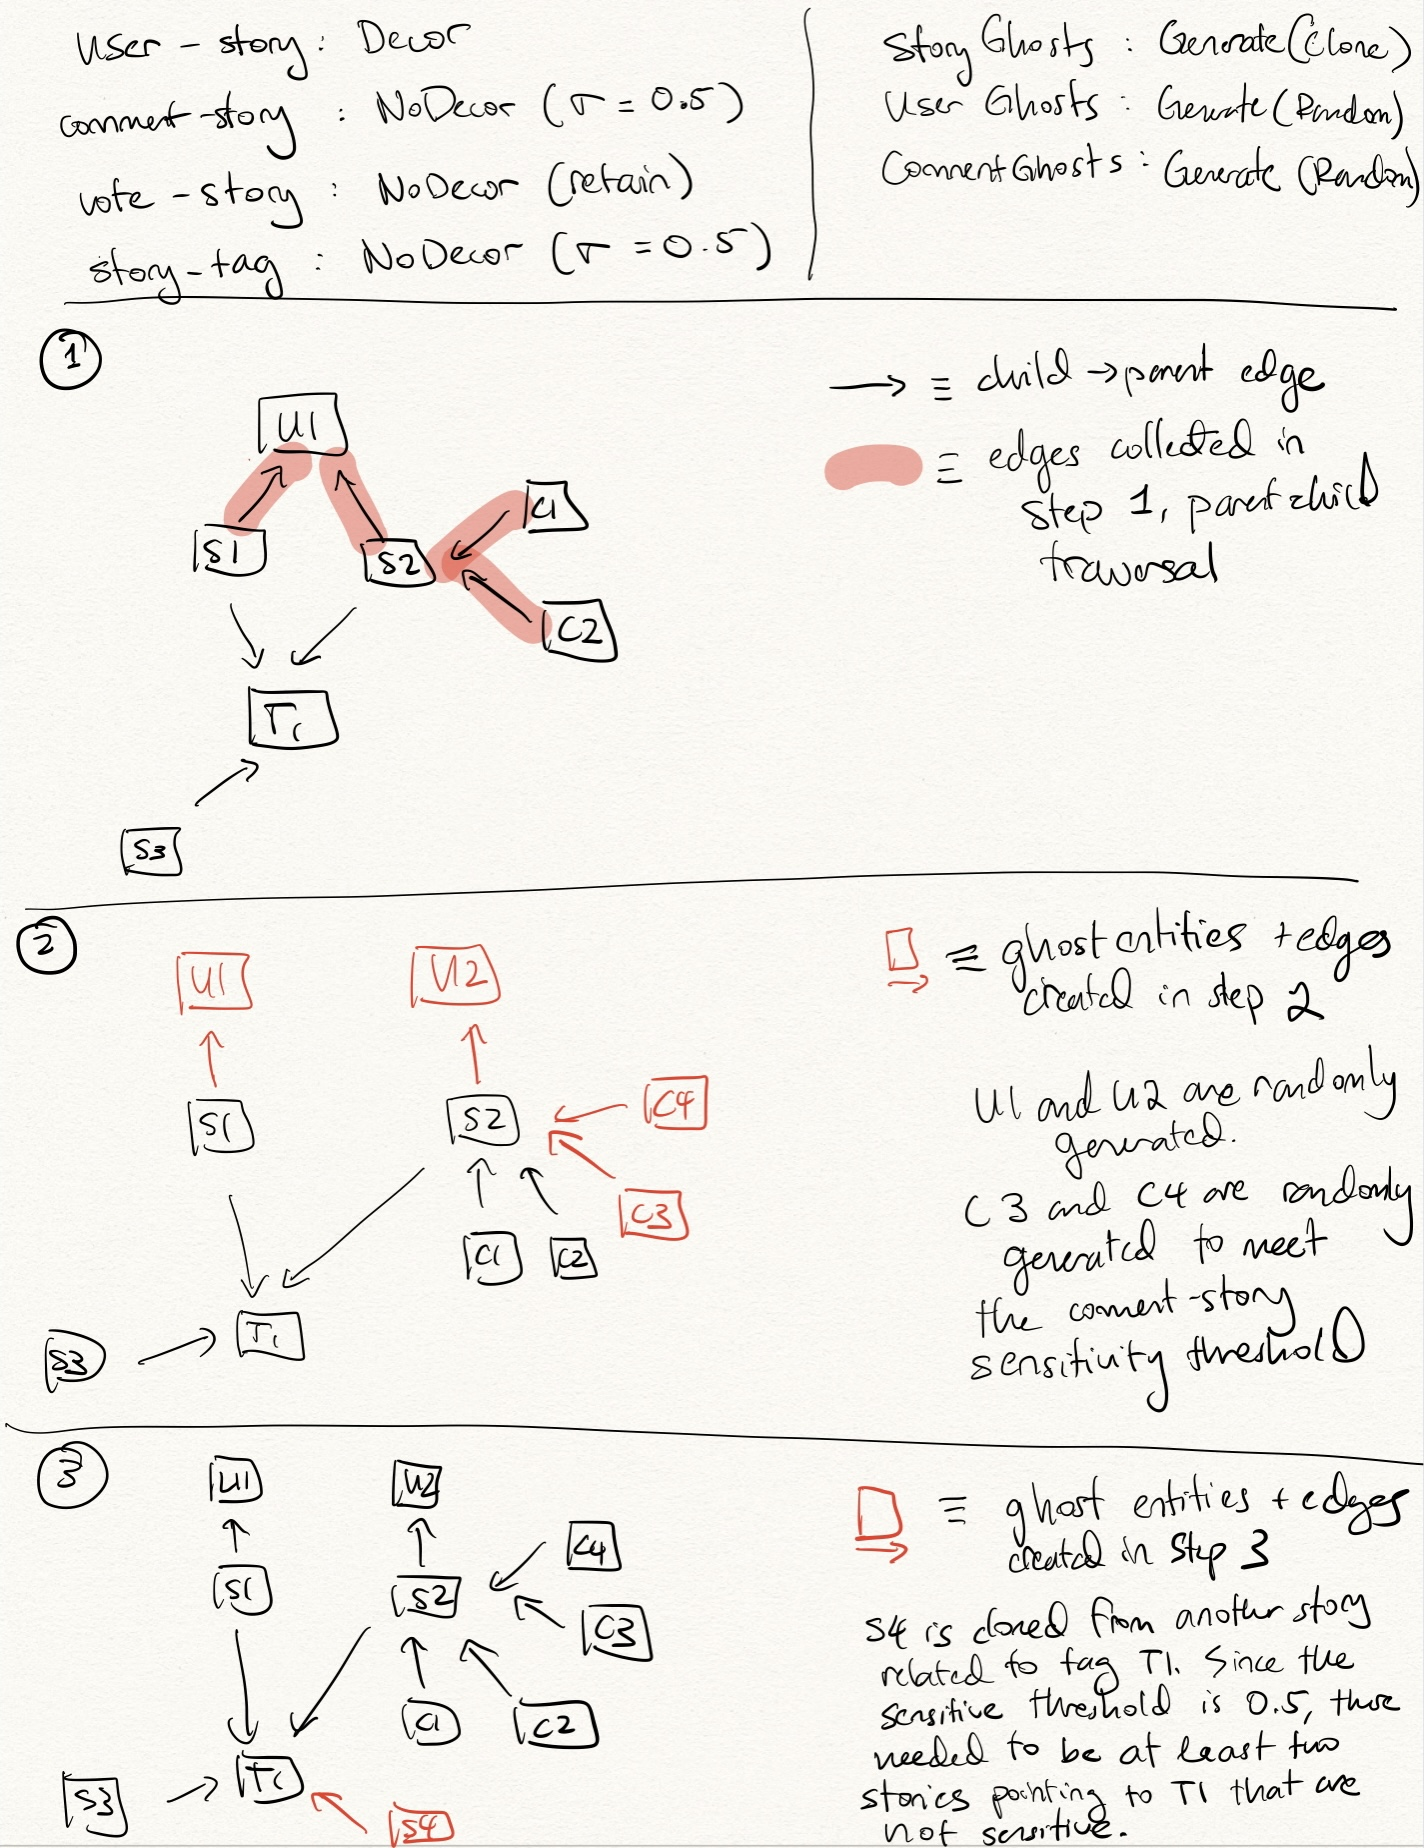
\includegraphics[width=.5\textwidth]{img/algo}
    \label{fig:algo}
    \caption{Examples of \sys{}'s execution.}
\end{figure}

%\paragraph{Example policy.}
%We can imagine an application tin which only the sum of votes per story is ever queried by the application; clusters of
%votes around stories can therefore remain without leaking identifying information, and are thus
%assigned Policy 1, ``Do Not Decorrelate (Retain)''. 
%Decorrelation does propagate to the votes themselves, which are clustered by a \texttt{location} attribute; 
%this cluster by location can have a different decorrelation policy that generates ghost locations by
%randomizing the location, breaking up the cluster. 
%
